\begin{table}[htbp]\centering\small

\begin{tabular}{lrrrrr}\toprule

Method & Successes/runs & $Q$ & Gates$^\dagger$ & Seconds & Edges \\ \midrule

Trained hierarchy & 130/300 & 0.160 & 4.54 & 0.758 & 1927 \\

Untrained prior & 24/60 & 0.149 & 4.58 & 0.772 & 2098 \\

Outer only & 137/300 & 0.163 & 4.66 & 0.748 & 2015 \\

Inner only & 125/300 & 0.153 & 4.65 & 0.758 & 2407 \\

Greedy & 26/60 & 0.164 & 4.62 & 0.754 & 2528 \\

Uniform cost & 22/60 & 0.142 & 4.55 & 0.754 & 8485 \\

Cold MITM & 51/60 & 0.308 & 4.78 & 0.232 & 4928 \\

\bottomrule\end{tabular}

\caption{One-second primary endpoint. $Q$ is the failure-aware native-gate resource score; $\dagger$ denotes successful runs only, which must not be interpreted without success rate. Learned variants use five training seeds and two timing repetitions; deterministic controls use two repetitions. Table entries include all executed jobs, not only successes.}\label{tab:primary}

\end{table}

The locked campaign contains 3,420 primary jobs on 30 distinct logical targets. At the primary one-second endpoint the hierarchy--prior difference in $Q$ is 0.0111, with a paired target-cluster 95\% interval [0.0000,0.0333]. The target, not a timing repetition or training seed, is the resampling unit.

The primary endpoint supports a positive target-average effect in this sampled domain; it does not establish superiority on other resource contracts or larger registers.

\begin{table}[htbp]\centering\small

\begin{tabular}{llrrr}\toprule

Budget axis & Budget & Hierarchy $Q$ & Prior $Q$ & Paired difference [95\%] \\ \midrule

Native edges & 128 & 0.060 & 0.055 & 0.005 [-0.029,0.038] \\

Native edges & 1024 & 0.119 & 0.119 & 0.001 [-0.023,0.029] \\

Wall seconds & 0.2 & 0.103 & 0.111 & -0.008 [-0.039,0.026] \\

Wall seconds & 1.0 & 0.160 & 0.149 & 0.011 [0.000,0.033] \\

\bottomrule\end{tabular}\caption{Budget-dependent comparisons. Only the one-second $Q$ contrast is primary; the other intervals are descriptive and unadjusted for multiple comparisons.}\label{tab:budgets}\end{table}

\begin{table}[htbp]\centering\small\begin{tabular}{lrrr}\toprule

Variant & Successes/runs & Mean $Q$ & Difference from full [95\%] \\ \midrule

full & 28/90 & 0.121 & -- \\

no\_inner\_bootstrap & 30/90 & 0.128 & 0.007 [-0.002,0.019] \\

frontier\_inner\_bootstrap & 27/90 & 0.117 & -0.004 [-0.017,0.008] \\

no\_structure & 31/90 & 0.130 & 0.009 [-0.008,0.034] \\

\bottomrule\end{tabular}\caption{Exploratory, independently retrained ablations at 1024 edges, with three matched training seeds. No variant is selected using these test results.}\label{tab:ablations}\end{table}

Off-policy withheld-prefix probes contain 30 states. The trained inner policies select an action with a verified two-gate completion in 65/150 selections; the prior does so in 15/30 probes. There are 5 probes with same-family feature vectors within $10^{-12}$ but different bounded completion outcomes, and 7 with a verified completion whose first step increases target discrepancy. These are diagnostic states from withheld construction prefixes after testing, not a claim about the policies' on-policy state distribution. Unresolved continuations are not labelled globally impossible.

On 12 fixed validation frontiers, full-frontier scoring selects a different record from panel scoring in 6 snapshots. Consequently, panel/full-frontier performance cannot be attributed solely to arithmetic overhead; the allowed policy selection set changes too. The microbenchmark records raw scoring with precomputed vectors separately.

Of the 12 predetermined post-campaign optimization problems, 8 close all requested native resource gaps and pass the separate exact cyclotomic verifier. Independent replay verifies 72 distinct saved discovery-circuit/contract pairs and 102 constructor specifications. Certificates and unchanged upper-bound/unknown outcomes are archived individually; these counts are not independent targets.

\begin{table}[htbp]\centering\small\begin{tabular}{lrrr}\toprule

Challenge family & Hierarchy & Prior & Cold MITM \\ \midrule

QFT & 0/6 & 0/6 & 3/6 \\

SWAP & 3/3 & 3/3 & 3/3 \\

Toffoli & 0/6 & 0/6 & 0/6 \\

ancilla-mixed-Pauli & 0/3 & 0/3 & 3/3 \\

phase-oracle & 0/25 & 0/25 & 0/25 \\

\bottomrule\end{tabular}\caption{Unchanged 43-contract challenge registry, three-second discovery-only limits and one frozen seed. This is not a broad generalization estimate. Known exact determinant obstructions are reported separately, not inferred from these time limits.}\label{tab:challenges}\end{table}

\begin{table}[htbp]\centering\small\begin{tabular}{lrrrrr}\toprule

Known one-clean-wire reference & $N_T$ & $N_{CX}$ & $D$ & $N_G$ & Min. clean width \\ \midrule

qft-3-clean-1 & 15 & 13 & 26 & 35 & 1 \\

toffoli-4-clean-1 & 21 & 18 & 33 & 45 & 1 \\

\bottomrule\end{tabular}\caption{Exact reference replay plus determinant exclusions establishes minimum clean width for these ideal exact-phase targets. These are existing constructions and are not learned discoveries or claims of gate optimality.}\label{tab:reach}\end{table}

\begin{table}[htbp]\centering\small\begin{tabular}{lrrrrrr}\toprule

Controlled-$S$ reference & Anc. & $N_T$ & $D_T$ & $N_{CX}$ & $D$ & $N_G$ \\ \midrule

Exact native word & 0 & 3 & 2 & 2 & 4 & 5 \\

Exact native word & 1 & 3 & 1 & 4 & 5 & 7 \\

\bottomrule\end{tabular}\caption{Known ancilla--$T$-depth trade-off, independently replayed. These witnesses are not used as native search inputs. No fixed-polynomial rank certificate is imported into the general native search domain.}\label{tab:cs}\end{table}

Native discovery finds a timely controlled-$S$ witness in 2/12 separately budgeted calibration attempts. The complete six-target, three-width crossed workspace study is archived; availability of an ancilla is not itself evidence that a policy uses it effectively.

For the new two-input threshold-network conjunction predicate, Trained hierarchy finds a certified oracle; Untrained prior finds a certified oracle; Cold MITM finds a certified oracle. All returned oracles are checked by exact promised-input replay and executed coherently with a diffusion operator. The ideal marked-state probability is one after one iteration. Diffusion cost is not included in the reported oracle resources; no large-BNN quantum advantage is claimed.

\begin{figure}[htbp]\centering\resizebox{\linewidth}{!}{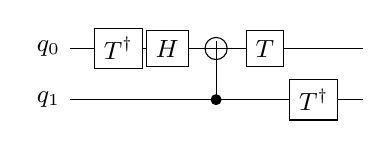
\begin{tikzpicture}[x=0.62cm,y=0.65cm, every node/.style={font=\small}]
\draw (0,0) node[left]{$q_0$} -- (6,0);
\draw (0,-1) node[left]{$q_1$} -- (6,-1);
\node[draw,fill=white,minimum size=0.43cm] at (1,0) {$ T^\dagger $};
\node[draw,fill=white,minimum size=0.43cm] at (2,0) {$ H $};
\draw (3,-1) -- (3,0);\fill (3,-1) circle (2pt);\draw (3,0) circle (4pt);\draw (3,0-.15)--(3,0+.15);
\node[draw,fill=white,minimum size=0.43cm] at (4,0) {$ T $};
\node[draw,fill=white,minimum size=0.43cm] at (5,-1) {$ T^\dagger $};
\end{tikzpicture}
}\caption{A circuit actually generated by the frozen native hierarchy for test-n2-14 (seed 47). Gate order comes directly from the saved native witness.}\label{fig:circuit}\end{figure}
